\documentclass[twocolumn]{article}
\usepackage{usenix}

%\documentclass[times,10pt,twocolumn]{article}
%\usepackage{latex8}
%\usepackage{times}
\usepackage{url}
\usepackage{graphics}
\usepackage{amsmath}
\usepackage{epsfig}

\pagestyle{empty}

\renewcommand\url{\begingroup \def\UrlLeft{<}\def\UrlRight{>}\urlstyle{tt}\Url}
\newcommand\emailaddr{\begingroup \def\UrlLeft{<}\def\UrlRight{>}\urlstyle{tt}\Url}

\newcommand{\workingnote}[1]{}        % The version that hides the note.
%\newcommand{\workingnote}[1]{(**#1)}   % The version that makes the note visible.

% If an URL ends up with '%'s in it, that's because the line *in the .bib/.tex
% file* is too long, so break it there (it doesn't matter if the next line is
% indented with spaces). -DH

%\newif\ifpdf
%\ifx\pdfoutput\undefined
%   \pdffalse
%\else
%   \pdfoutput=1
%   \pdftrue
%\fi

\newenvironment{tightlist}{\begin{list}{$\bullet$}{
  \setlength{\itemsep}{0mm}
    \setlength{\parsep}{0mm}
    %  \setlength{\labelsep}{0mm}
    %  \setlength{\labelwidth}{0mm}
    %  \setlength{\topsep}{0mm}
    }}{\end{list}}

% Cut down on whitespace above and below figures displayed at head/foot of
% page.
\setlength{\textfloatsep}{3mm}
% Cut down on whitespace above and below figures displayed in middle of page
\setlength{\intextsep}{3mm}

\begin{document}

%% Use dvipdfm instead. --DH
%\ifpdf
%  \pdfcompresslevel=9
%  \pdfpagewidth=\the\paperwidth
%  \pdfpageheight=\the\paperheight
%\fi

\title{Tor: The Second-Generation Onion Router} %\\DRAFT VERSION}
% Putting the 'Private' back in 'Virtual Private Network'

\author{Roger Dingledine \\ The Free Haven Project \\ arma@freehaven.net \and
Nick Mathewson \\ The Free Haven Project \\ nickm@freehaven.net \and
Paul Syverson \\ Naval Research Lab \\ syverson@itd.nrl.navy.mil}

\maketitle
\thispagestyle{empty}

\begin{abstract}
We present Tor, a circuit-based low-latency anonymous communication
service. This second-generation Onion Routing system addresses limitations
in the original design. Tor adds perfect forward secrecy, congestion
control, directory servers, integrity checking, configurable exit policies,
and a practical design for location-hidden services via rendezvous
points. Tor works on the real-world
Internet, requires no special privileges or kernel modifications, requires
little synchronization or coordination between nodes, and provides a
reasonable tradeoff between anonymity, usability, and efficiency.
We briefly describe our experiences with an international network of
more than 30 nodes. % that has been running for several months.
We close with a list of open problems in anonymous communication.
\end{abstract}

%\begin{center}
%\textbf{Keywords:} anonymity, peer-to-peer, remailer, nymserver, reply block
%\end{center}

%%%%%%%%%%%%%%%%%%%%%%%%%%%%%%%%%%%%%%%%%%%%%%%%%%%%%%%%%%%%%%%%%%%%%%%

\section{Overview}
\label{sec:intro}

Onion Routing is a distributed overlay network designed to anonymize
TCP-based applications like web browsing, secure shell,
and instant messaging. Clients choose a path through the network and
build a \emph{circuit}, in which each node (or ``onion router'' or ``OR'')
in the path knows its predecessor and successor, but no other nodes in
the circuit.  Traffic flows down the circuit in fixed-size
\emph{cells}, which are unwrapped by a symmetric key at each node
(like the layers of an onion) and relayed downstream. The
Onion Routing project published several design and analysis
papers \cite{or-ih96,or-jsac98,or-discex00,or-pet00}. While a wide area Onion
Routing network was deployed briefly, the only long-running
public implementation was a fragile
proof-of-concept that ran on a single machine. Even this simple deployment
processed connections from over sixty thousand distinct IP addresses from
all over the world at a rate of about fifty thousand per day.
But many critical design and deployment issues were never
resolved, and the design has not been updated in several years. Here
we describe Tor, a protocol for asynchronous, loosely federated onion
routers that provides the following improvements over the old Onion
Routing design:

\textbf{Perfect forward secrecy:} In the original Onion Routing design,
a single hostile node could record traffic and
later compromise successive nodes in the circuit and force them
to decrypt it. Rather than using a single multiply encrypted data
structure (an \emph{onion}) to lay each circuit,
Tor now uses an incremental or \emph{telescoping} path-building design,
where the initiator negotiates session keys with each successive hop in
the circuit.  Once these keys are deleted, subsequently compromised nodes
cannot decrypt old traffic.  As a side benefit, onion replay detection
is no longer necessary, and the process of building circuits is more
reliable, since the initiator knows when a hop fails and can then try
extending to a new node.

\textbf{Separation of ``protocol cleaning'' from anonymity:}
Onion Routing originally required a separate ``application
proxy'' for each supported application protocol---most of which were
never written, so many applications were never supported.  Tor uses the
standard and near-ubiquitous SOCKS~\cite{socks4} proxy interface, allowing
us to support most TCP-based programs without modification.  Tor now
relies on the filtering features of privacy-enhancing
application-level proxies such as Privoxy~\cite{privoxy}, without trying
to duplicate those features itself.

\textbf{No mixing, padding, or traffic shaping (yet):} Onion
Routing originally called for batching and reordering cells as they arrived,
assumed padding between ORs, and in
later designs added padding between onion proxies (users) and
ORs~\cite{or-ih96,or-jsac98}.  Tradeoffs between padding protection
and cost were discussed, and \emph{traffic shaping} algorithms were
theorized~\cite{or-pet00} to provide good security without expensive
padding, but no concrete padding scheme was suggested.
Recent research~\cite{econymics}
and deployment experience~\cite{freedom21-security} suggest that this
level of resource use is not practical or economical; and even full
link padding is still vulnerable~\cite{defensive-dropping}. Thus,
until we have a proven and convenient design for traffic shaping or
low-latency mixing that improves anonymity against a realistic
adversary, we leave these strategies out.

\textbf{Many TCP streams can share one circuit:} Onion Routing originally
built a separate circuit for each
application-level request, but this required
multiple public key operations for every request, and also presented
a threat to anonymity from building so many circuits; see
Section~\ref{sec:maintaining-anonymity}.  Tor multiplexes multiple TCP
streams along each circuit to improve efficiency and anonymity.

\textbf{Leaky-pipe circuit topology:} Through in-band signaling
within the circuit, Tor initiators can direct traffic to nodes partway
down the circuit. This novel approach
allows traffic to exit the circuit from the middle---possibly
frustrating traffic shape and volume attacks based on observing the end
of the circuit. (It also allows for long-range padding if
future research shows this to be worthwhile.)

\textbf{Congestion control:} Earlier anonymity designs do not
address traffic bottlenecks. Unfortunately, typical approaches to
load balancing and flow control in overlay networks involve inter-node
control communication and global views of traffic. Tor's decentralized
congestion control uses end-to-end acks to maintain anonymity
while allowing nodes at the edges of the network to detect congestion
or flooding and send less data until the congestion subsides.

\textbf{Directory servers:} The earlier Onion Routing design
planned to flood state information through the network---an approach
that can be unreliable and complex. % open to partitioning attacks.
Tor takes a simplified view toward distributing this
information. Certain more trusted nodes act as \emph{directory
servers}: they provide signed directories describing known
routers and their current state. Users periodically download them
via HTTP.

\textbf{Variable exit policies:} Tor provides a consistent mechanism
for each node to advertise a policy describing the hosts
and ports to which it will connect. These exit policies are critical
in a volunteer-based distributed infrastructure, because each operator
is comfortable with allowing different types of traffic to exit
from his node.

\textbf{End-to-end integrity checking:} The original Onion Routing
design did no integrity checking on data. Any node on the
circuit could change the contents of data cells as they passed by---for
example, to alter a connection request so it would connect
to a different webserver, or to `tag' encrypted traffic and look for
corresponding corrupted traffic at the network edges~\cite{minion-design}.
Tor hampers these attacks by verifying data integrity before it leaves
the network.

%\textbf{Improved robustness to failed nodes:} A failed node
%in the old design meant that circuit building failed, but thanks to
%Tor's step-by-step circuit building, users notice failed nodes
%while building circuits and route around them. Additionally, liveness
%information from directories allows users to avoid unreliable nodes in
%the first place.
%% Can't really claim this, now that we've found so many variants of
%% attack on partial-circuit-building. -RD

\textbf{Rendezvous points and hidden services:}
Tor provides an integrated mechanism for responder anonymity via
location-protected servers.  Previous Onion Routing designs included
long-lived ``reply onions'' that could be used to build circuits
to a hidden server, but these reply onions did not provide forward
security, and became useless if any node in the path went down
or rotated its keys.  In Tor, clients negotiate {\it rendezvous points}
to connect with hidden servers; reply onions are no longer required.

Unlike Freedom~\cite{freedom2-arch}, Tor does not require OS kernel
patches or network stack support.  This prevents us from anonymizing
non-TCP protocols, but has greatly helped our portability and
deployability.

%Unlike Freedom~\cite{freedom2-arch}, Tor only anonymizes
%TCP-based protocols---not requiring patches (or built-in support) in an
%operating system's network stack has been valuable to Tor's
%portability and deployability.

We have implemented all of the above features, including rendezvous
points. Our source code is
available under a free license, and Tor
%, as far as we know, is unencumbered by patents.
is not covered by the patent that affected distribution and use of
earlier versions of Onion Routing.
We have deployed a wide-area alpha network
to test the design, to get more experience with usability
and users, and to provide a research platform for experimentation.
As of this writing, the network stands at 32 nodes %in thirteen
%distinct administrative domains
spread over two continents.

We review previous work in Section~\ref{sec:related-work}, describe
our goals and assumptions in Section~\ref{sec:assumptions},
and then address the above list of improvements in
Sections~\ref{sec:design},~\ref{sec:rendezvous}, and~\ref{sec:other-design}.
We summarize
in Section~\ref{sec:attacks} how our design stands up to
known attacks, and talk about our early deployment experiences in
Section~\ref{sec:in-the-wild}. We conclude with a list of open problems in
Section~\ref{sec:maintaining-anonymity} and future work for the Onion
Routing project in Section~\ref{sec:conclusion}.

%%%%%%%%%%%%%%%%%%%%%%%%%%%%%%%%%%%%%%%%%%%%%%%%%%%%%%%%%%%%%%%%%%%%%%%

\section{Related work}
\label{sec:related-work}

Modern anonymity systems date to Chaum's {\bf Mix-Net}
design~\cite{chaum-mix}. Chaum
proposed hiding the correspondence between sender and recipient by
wrapping messages in layers of public-key cryptography, and relaying them
through a path composed of ``mixes.''  Each mix in turn
decrypts, delays, and re-orders messages before relaying them
onward.
%toward their destinations.

Subsequent relay-based anonymity designs have diverged in two
main directions. Systems like {\bf Babel}~\cite{babel},
{\bf Mixmaster}~\cite{mixmaster-spec},
and {\bf Mixminion}~\cite{minion-design} have tried
to maximize anonymity at the cost of introducing comparatively large and
variable latencies. Because of this decision, these \emph{high-latency}
networks resist strong global adversaries,
but introduce too much lag for interactive tasks like web browsing,
Internet chat, or SSH connections.

Tor belongs to the second category: \emph{low-latency} designs that
try to anonymize interactive network traffic. These systems handle
a variety of bidirectional protocols. They also provide more convenient
mail delivery than the high-latency anonymous email
networks, because the remote mail server provides explicit and timely
delivery confirmation. But because these designs typically
involve many packets that must be delivered quickly, it is
difficult for them to prevent an attacker who can eavesdrop both ends of the
communication from correlating the timing and volume
of traffic entering the anonymity network with traffic leaving it~\cite{SS03}.
These
protocols are similarly vulnerable to an active adversary who introduces
timing patterns into traffic entering the network and looks
for correlated patterns among exiting traffic.
Although some work has been done to frustrate these attacks, most designs
protect primarily against traffic analysis rather than traffic
confirmation (see Section~\ref{subsec:threat-model}).

The simplest low-latency designs are single-hop proxies such as the
{\bf Anonymizer}~\cite{anonymizer}: a single trusted server strips the
data's origin before relaying it.  These designs are easy to
analyze, but users must trust the anonymizing proxy.
Concentrating the traffic to this single point increases the anonymity set
(the people a given user is hiding among), but it is vulnerable if the
adversary can observe all traffic entering and leaving the proxy.

More complex are distributed-trust, circuit-based anonymizing systems.
In these designs, a user establishes one or more medium-term bidirectional
end-to-end circuits, and tunnels data in fixed-size cells.
Establishing circuits is computationally expensive and typically
requires public-key
cryptography, whereas relaying cells is comparatively inexpensive and
typically requires only symmetric encryption.
Because a circuit crosses several servers, and each server only knows
the adjacent servers in the circuit, no single server can link a
user to her communication partners.

The {\bf Java Anon Proxy} (also known as JAP or Web MIXes) uses fixed shared
routes known as \emph{cascades}.  As with a single-hop proxy, this
approach aggregates users into larger anonymity sets, but again an
attacker only needs to observe both ends of the cascade to bridge all
the system's traffic.  The Java Anon Proxy's design
calls for padding between end users and the head of the
cascade~\cite{web-mix}. However, it is not demonstrated whether the current
implementation's padding policy improves anonymity.

{\bf PipeNet}~\cite{back01, pipenet}, another low-latency design proposed
around the same time as Onion Routing, gave
stronger anonymity but allowed a single user to shut
down the network by not sending. Systems like {\bf ISDN
mixes}~\cite{isdn-mixes} were designed for other environments with
different assumptions.
%XXX please can we fix this sentence to something less demeaning

In P2P designs like {\bf Tarzan}~\cite{tarzan:ccs02} and
{\bf MorphMix}~\cite{morphmix:fc04}, all participants both generate
traffic and relay traffic for others. These systems aim to conceal
whether a given peer originated a request
or just relayed it from another peer. While Tarzan and MorphMix use
layered encryption as above, {\bf Crowds}~\cite{crowds-tissec} simply assumes
an adversary who cannot observe the initiator: it uses no public-key
encryption, so any node on a circuit can read users' traffic.

{\bf Hordes}~\cite{hordes-jcs} is based on Crowds but also uses multicast
responses to hide the initiator. {\bf Herbivore}~\cite{herbivore} and
$\mbox{\bf P}^{\mathbf 5}$~\cite{p5} go even further, requiring broadcast.
These systems are designed primarily for communication among peers,
although Herbivore users can make external connections by
requesting a peer to serve as a proxy.

Systems like {\bf Freedom} and the original Onion Routing build circuits
all at once, using a layered ``onion'' of public-key encrypted messages,
each layer of which provides session keys and the address of the
next server in the circuit. Tor as described herein, Tarzan, MorphMix,
{\bf Cebolla}~\cite{cebolla}, and Rennhard's {\bf Anonymity Network}~\cite{anonnet}
build circuits
in stages, extending them one hop at a time.
Section~\ref{subsubsec:constructing-a-circuit} describes how this
approach enables perfect forward secrecy.

Circuit-based anonymity designs must choose which protocol layer
to anonymize. They may choose to intercept IP packets directly, and
relay them whole (stripping the source address) along the
circuit~\cite{freedom2-arch,tarzan:ccs02}.  Alternatively, like
Tor, they may accept TCP streams and relay the data in those streams
along the circuit, ignoring the breakdown of that data into TCP
segments~\cite{morphmix:fc04,anonnet}. Finally, they may accept
application-level protocols (such as HTTP) and relay the application
requests themselves along the circuit.
Making this protocol-layer decision requires a compromise between flexibility
and anonymity.  For example, a system that understands HTTP, such as Crowds,
can strip
identifying information from those requests, can take advantage of caching
to limit the number of requests that leave the network, and can batch
or encode those requests to minimize the number of connections.
On the other hand, an IP-level anonymizer can handle nearly any protocol,
even ones unforeseen by its designers (though these systems require
kernel-level modifications to some operating systems, and so are more
complex and less portable). TCP-level anonymity networks like Tor present
a middle approach: they are fairly application neutral (so long as the
application supports, or can be tunneled across, TCP), but by treating
application connections as data streams rather than raw TCP packets,
they avoid the well-known inefficiencies of tunneling TCP over
TCP~\cite{tcp-over-tcp-is-bad}.

Distributed-trust anonymizing systems need to prevent attackers from
adding too many servers and thus compromising user paths.
Tor relies on a small set of well-known directory servers, run by
independent parties, to decide which nodes can
join. Tarzan and MorphMix allow unknown users to run servers, and use
a limited resource (like IP addresses) to prevent an attacker from
controlling too much of the network.  Crowds suggests requiring
written, notarized requests from potential crowd members.

Anonymous communication is essential for censorship-resistant
systems like Eternity~\cite{eternity}, Free~Haven~\cite{freehaven-berk},
Publius~\cite{publius}, and Tangler~\cite{tangler}. Tor's rendezvous
points enable connections between mutually anonymous entities; they
are a building block for location-hidden servers, which are needed by
Eternity and Free~Haven.

% didn't include rewebbers. No clear place to put them, so I'll leave
% them out for now. -RD

\section{Design goals and assumptions}
\label{sec:assumptions}

\noindent{\large\bf Goals}\\
Like other low-latency anonymity designs, Tor seeks to frustrate
attackers from linking communication partners, or from linking
multiple communications to or from a single user.  Within this
main goal, however, several considerations have directed
Tor's evolution.

\textbf{Deployability:} The design must be deployed and used in the
real world.  Thus it
must not be expensive to run (for example, by requiring more bandwidth
than volunteers are willing to provide); must not place a heavy
liability burden on operators (for example, by allowing attackers to
implicate onion routers in illegal activities); and must not be
difficult or expensive to implement (for example, by requiring kernel
patches, or separate proxies for every protocol).  We also cannot
require non-anonymous parties (such as websites)
to run our software.  (Our rendezvous point design does not meet
this goal for non-anonymous users talking to hidden servers,
however; see Section~\ref{sec:rendezvous}.)

\textbf{Usability:} A hard-to-use system has fewer users---and because
anonymity systems hide users among users, a system with fewer users
provides less anonymity.  Usability is thus not only a convenience:
it is a security requirement~\cite{econymics,back01}. Tor should
therefore not
require modifying familiar applications; should not introduce prohibitive
delays;
and should require as few configuration decisions
as possible.  Finally, Tor should be easily implementable on all common
platforms; we cannot require users to change their operating system
to be anonymous.  (The current Tor implementation runs on Windows and
assorted Unix clones including Linux, FreeBSD, and MacOS X.)

\textbf{Flexibility:} The protocol must be flexible and well-specified,
so Tor can serve as a test-bed for future research.
Many of the open problems in low-latency anonymity
networks, such as generating dummy traffic or preventing Sybil
attacks~\cite{sybil}, may be solvable independently from the issues
solved by
Tor. Hopefully future systems will not need to reinvent Tor's design.
%(But note that while a flexible design benefits researchers,
%there is a danger that differing choices of extensions will make users
%distinguishable. Experiments should be run on a separate network.)

\textbf{Simple design:} The protocol's design and security
parameters must be well-understood. Additional features impose implementation
and complexity costs; adding unproven techniques to the design threatens
deployability, readability, and ease of security analysis. Tor aims to
deploy a simple and stable system that integrates the best accepted
approaches to protecting anonymity.\\

\noindent{\large\bf Non-goals}\label{subsec:non-goals}\\
In favoring simple, deployable designs, we have explicitly deferred
several possible goals, either because they are solved elsewhere, or because
they are not yet solved.

\textbf{Not peer-to-peer:} Tarzan and MorphMix aim to scale to completely
decentralized peer-to-peer environments with thousands of short-lived
servers, many of which may be controlled by an adversary.  This approach
is appealing, but still has many open
problems~\cite{tarzan:ccs02,morphmix:fc04}.

\textbf{Not secure against end-to-end attacks:} Tor does not claim
to provide a definitive solution to end-to-end timing or intersection
attacks. Some approaches, such as having users run their own onion routers, 
may help;
see Section~\ref{sec:maintaining-anonymity} for more discussion.

\textbf{No protocol normalization:} Tor does not provide \emph{protocol
normalization} like Privoxy or the Anonymizer. If senders want anonymity from
responders while using complex and variable
protocols like HTTP, Tor must be layered with a filtering proxy such
as Privoxy to hide differences between clients, and expunge protocol
features that leak identity.
Note that by this separation Tor can also provide services that
are anonymous to the network yet authenticated to the responder, like
SSH. Similarly, Tor does not integrate
tunneling for non-stream-based protocols like UDP; this must be
provided by an external service if appropriate.

\textbf{Not steganographic:} Tor does not try to conceal who is connected
to the network.

\subsection{Threat Model}
\label{subsec:threat-model}

A global passive adversary is the most commonly assumed threat when
analyzing theoretical anonymity designs. But like all practical
low-latency systems, Tor does not protect against such a strong
adversary. Instead, we assume an adversary who can observe some fraction
of network traffic; who can generate, modify, delete, or delay
traffic;  who can operate onion routers of his own; and who can
compromise some fraction of the onion routers.

In low-latency anonymity systems that use layered encryption, the
adversary's typical goal is to observe both the initiator and the
responder. By observing both ends, passive attackers can confirm a
suspicion that Alice is
talking to Bob if the timing and volume patterns of the traffic on the
connection are distinct enough; active attackers can induce timing
signatures on the traffic to force distinct patterns. Rather
than focusing on these \emph{traffic confirmation} attacks,
we aim to prevent \emph{traffic
analysis} attacks, where the adversary uses traffic patterns to learn
which points in the network he should attack.

Our adversary might try to link an initiator Alice with her
communication partners, or try to build a profile of Alice's
behavior. He might mount passive attacks by observing the network edges
and correlating traffic entering and leaving the network---by
relationships in packet timing, volume, or externally visible
user-selected
options. The adversary can also mount active attacks by compromising
routers or keys; by replaying traffic; by selectively denying service
to trustworthy routers to move users to
compromised routers, or denying service to users to see if traffic
elsewhere in the
network stops; or by introducing patterns into traffic that can later be
detected. The adversary might subvert the directory servers to give users
differing views of network state. Additionally, he can try to decrease
the network's reliability by attacking nodes or by performing antisocial
activities from reliable nodes and trying to get them taken down---making
the network unreliable flushes users to other less anonymous
systems, where they may be easier to attack. We summarize
in Section~\ref{sec:attacks} how well the Tor design defends against
each of these attacks.

%%%%%%%%%%%%%%%%%%%%%%%%%%%%%%%%%%%%%%%%%%%%%%%%%%%%%%%%%%%%%%%%%%%%%%%

\section{The Tor Design}
\label{sec:design}

The Tor network is an overlay network; each onion router (OR)
runs as a normal
user-level process without any special privileges.
Each onion router maintains a TLS~\cite{TLS}
connection to every other onion router.
%(We discuss alternatives to this clique-topology assumption in
%Section~\ref{sec:maintaining-anonymity}.)
% A subset of the ORs also act as
%directory servers, tracking which routers are in the network;
%see Section~\ref{subsec:dirservers} for directory server details.
Each user
runs local software called an onion proxy (OP) to fetch directories,
establish circuits across the network,
and handle connections from user applications.  These onion proxies accept
TCP streams and multiplex them across the circuits. The onion
router on the other side
of the circuit connects to the requested destinations
and relays data.

Each onion router maintains a long-term identity key and a short-term
onion key. The identity
key is used to sign TLS certificates, to sign the OR's \emph{router
descriptor} (a summary of its keys, address, bandwidth, exit policy,
and so on), and (by directory servers) to sign directories. %Changing
%the identity key of a router is considered equivalent to creating a
%new router. 
The onion key is used to decrypt requests
from users to set up a circuit and negotiate ephemeral keys. 
The TLS protocol also establishes a short-term link key when communicating
between ORs. Short-term keys are rotated periodically and
independently, to limit the impact of key compromise.

Section~\ref{subsec:cells} presents the fixed-size
\emph{cells} that are the unit of communication in Tor. We describe
in Section~\ref{subsec:circuits} how circuits are
built, extended, truncated, and destroyed. Section~\ref{subsec:tcp}
describes how TCP streams are routed through the network.  We address
integrity checking in Section~\ref{subsec:integrity-checking},
and resource limiting in Section~\ref{subsec:rate-limit}.
Finally,
Section~\ref{subsec:congestion} talks about congestion control and
fairness issues.

\subsection{Cells}
\label{subsec:cells}

Onion routers communicate with one another, and with users' OPs, via
TLS connections with ephemeral keys.  Using TLS conceals the data on
the connection with perfect forward secrecy, and prevents an attacker
from modifying data on the wire or impersonating an OR.

Traffic passes along these connections in fixed-size cells.  Each cell
is 512 bytes, %(but see Section~\ref{sec:conclusion} for a discussion of
%allowing large cells and small cells on the same network),
and consists of a header and a payload. The header includes a circuit
identifier (circID) that specifies which circuit the cell refers to
(many circuits can be multiplexed over the single TLS connection), and
a command to describe what to do with the cell's payload.  (Circuit
identifiers are connection-specific: each circuit has a different
circID on each OP/OR or OR/OR connection it traverses.)
Based on their command, cells are either \emph{control} cells, which are
always interpreted by the node that receives them, or \emph{relay} cells,
which carry end-to-end stream data.   The control cell commands are:
\emph{padding} (currently used for keepalive, but also usable for link
padding); \emph{create} or \emph{created} (used to set up a new circuit);
and \emph{destroy} (to tear down a circuit).

Relay cells have an additional header (the relay header) at the front
of the payload, containing a streamID (stream identifier: many streams can
be multiplexed over a circuit); an end-to-end checksum for integrity
checking; the length of the relay payload; and a relay command.
The entire contents of the relay header and the relay cell payload
are encrypted or decrypted together as the relay cell moves along the
circuit, using the 128-bit AES cipher in counter mode to generate a
cipher stream.  The relay commands are: \emph{relay
data} (for data flowing down the stream), \emph{relay begin} (to open a
stream), \emph{relay end} (to close a stream cleanly), \emph{relay
teardown} (to close a broken stream), \emph{relay connected}
(to notify the OP that a relay begin has succeeded), \emph{relay
extend} and \emph{relay extended} (to extend the circuit by a hop,
and to acknowledge), \emph{relay truncate} and \emph{relay truncated}
(to tear down only part of the circuit, and to acknowledge), \emph{relay
sendme} (used for congestion control), and \emph{relay drop} (used to
implement long-range dummies).
We give a visual overview of cell structure plus the details of relay
cell structure, and then describe each of these cell types and commands
in more detail below.

\begin{figure}[h]
\unitlength=1cm
\centering
\begin{picture}(8.0,1.5)
\put(4,.5){\makebox(0,0)[c]{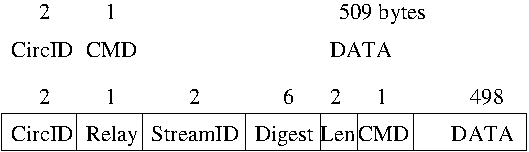
\epsfig{file=cell-struct,width=7cm}}}
\end{picture}
\end{figure}

\subsection{Circuits and streams}
\label{subsec:circuits}

Onion Routing originally built one circuit for each
TCP stream.  Because building a circuit can take several tenths of a
second (due to public-key cryptography and network latency),
this design imposed high costs on applications like web browsing that
open many TCP streams.

In Tor, each circuit can be shared by many TCP streams.  To avoid
delays, users construct circuits preemptively.  To limit linkability
among their streams, users' OPs build a new circuit
periodically if the previous ones have been used,
and expire old used circuits that no longer have any open streams.
OPs consider rotating to a new circuit once a minute: thus
even heavy users spend negligible time
building circuits, but a limited number of requests can be linked
to each other through a given exit node. Also, because circuits are built
in the background, OPs can recover from failed circuit creation
without delaying streams and thereby harming user experience.\\

\begin{figure}[h]
\centering
\mbox{\epsfig{figure=interaction,width=8.75cm}}
\caption{Alice builds a two-hop circuit and begins fetching a web page.}
\label{fig:interaction}
\end{figure}

\noindent{\large\bf Constructing a circuit}\label{subsubsec:constructing-a-circuit}\\
%\subsubsection{Constructing a circuit}
A user's OP constructs circuits incrementally, negotiating a
symmetric key with each OR on the circuit, one hop at a time. To begin
creating a new circuit, the OP (call her Alice) sends a
\emph{create} cell to the first node in her chosen path (call him Bob).
(She chooses a new
circID $C_{AB}$ not currently used on the connection from her to Bob.)
The \emph{create} cell's
payload contains the first half of the Diffie-Hellman handshake
($g^x$), encrypted to the onion key of the OR (call him Bob). Bob
responds with a \emph{created} cell containing the second half of the
DH handshake, along with a hash of the negotiated key $K=g^{xy}$.

Once the circuit has been established, Alice and Bob can send one
another relay cells encrypted with the negotiated
key.\footnote{Actually, the negotiated key is used to derive two
  symmetric keys: one for each direction.}  More detail is given in
the next section.

To extend the circuit further, Alice sends a \emph{relay extend} cell
to Bob, specifying the address of the next OR (call her Carol), and
an encrypted $g^{x_2}$ for her.  Bob copies the half-handshake into a
\emph{create} cell, and passes it to Carol to extend the circuit.
(Bob chooses a new circID $C_{BC}$ not currently used on the connection
between him and Carol.  Alice never needs to know this circID; only Bob
associates $C_{AB}$ on his connection with Alice to $C_{BC}$ on
his connection with Carol.)
When Carol responds with a \emph{created} cell, Bob wraps the payload
into a \emph{relay extended} cell and passes it back to Alice.  Now
the circuit is extended to Carol, and Alice and Carol share a common key
$K_2 = g^{x_2 y_2}$.

To extend the circuit to a third node or beyond, Alice
proceeds as above, always telling the last node in the circuit to
extend one hop further.

This circuit-level handshake protocol achieves unilateral entity
authentication (Alice knows she's handshaking with the OR, but
the OR doesn't care who is opening the circuit---Alice uses no public key
and is trying to remain anonymous) and unilateral key authentication
(Alice and the OR agree on a key, and Alice knows only the OR learns
it). It also achieves forward
secrecy and key freshness. More formally, the protocol is as follows
(where $E_{PK_{Bob}}(\cdot)$ is encryption with Bob's public key,
$H$ is a secure hash function, and $|$ is concatenation):
\begin{equation*}
\begin{aligned}
\mathrm{Alice} \rightarrow \mathrm{Bob}&: E_{PK_{Bob}}(g^x) \\
\mathrm{Bob} \rightarrow \mathrm{Alice}&: g^y, H(K | \mathrm{``handshake"}) \\
\end{aligned}
\end{equation*}

\noindent In the second step, Bob proves that it was he who received $g^x$,
and who chose $y$. We use PK encryption in the first step
(rather than, say, using the first two steps of STS, which has a
signature in the second step) because a single cell is too small to
hold both a public key and a signature. Preliminary analysis with the
NRL protocol analyzer~\cite{meadows96} shows this protocol to be
secure (including perfect forward secrecy) under the
traditional Dolev-Yao model.\\

\noindent{\large\bf Relay cells}\\
%\subsubsection{Relay cells}
%
Once Alice has established the circuit (so she shares keys with each
OR on the circuit), she can send relay cells.
%Recall that every relay cell has a streamID that indicates to which
%stream the cell belongs.  %This streamID allows a relay cell to be
%addressed to any OR on the circuit.  
Upon receiving a relay
cell, an OR looks up the corresponding circuit, and decrypts the relay
header and payload with the session key for that circuit.
If the cell is headed away from Alice the OR then checks whether the
decrypted cell has a valid digest (as an optimization, the first
two bytes of the integrity check are zero, so we only need to compute
the hash if the first two bytes are zero).
%is recognized---either because it
%corresponds to an open stream at this OR for the given circuit, or because
%it is the control streamID (zero).
If valid, it accepts the relay cell and processes it as described
below.  Otherwise,
the OR looks up the circID and OR for the
next step in the circuit, replaces the circID as appropriate, and
sends the decrypted relay cell to the next OR.  (If the OR at the end
of the circuit receives an unrecognized relay cell, an error has
occurred, and the circuit is torn down.)

OPs treat incoming relay cells similarly: they iteratively unwrap the
relay header and payload with the session keys shared with each
OR on the circuit, from the closest to farthest.
If at any stage the digest is valid, the cell must have
originated at the OR whose encryption has just been removed.

To construct a relay cell addressed to a given OR, Alice assigns the
digest, and then iteratively
encrypts the cell payload (that is, the relay header and payload) with
the symmetric key of each hop up to that OR.  Because the digest is
encrypted to a different value at each step, only at the targeted OR
will it have a meaningful value.\footnote{
  % Should we just say that 2^56 is itself negligible?
  % Assuming 4-hop circuits with 10 streams per hop, there are 33
  % possible bad streamIDs before the last circuit.  This still
  % gives an error only once every 2 million terabytes (approx).
With 48 bits of digest per cell, the probability of an accidental
collision is far lower than the chance of hardware failure.}
This \emph{leaky pipe} circuit topology
allows Alice's streams to exit at different ORs on a single circuit.
Alice may choose different exit points because of their exit policies,
or to keep the ORs from knowing that two streams
originate from the same person.

When an OR later replies to Alice with a relay cell, it
encrypts the cell's relay header and payload with the single key it
shares with Alice, and sends the cell back toward Alice along the
circuit.  Subsequent ORs add further layers of encryption as they
relay the cell back to Alice.

To tear down a circuit, Alice sends a \emph{destroy} control
cell. Each OR in the circuit receives the \emph{destroy} cell, closes
all streams on that circuit, and passes a new \emph{destroy} cell
forward. But just as circuits are built incrementally, they can also
be torn down incrementally: Alice can send a \emph{relay
truncate} cell to a single OR on a circuit. That OR then sends a
\emph{destroy} cell forward, and acknowledges with a
\emph{relay truncated} cell. Alice can then extend the circuit to
different nodes, without signaling to the intermediate nodes (or
a limited observer) that she has changed her circuit.
Similarly, if a node on the circuit goes down, the adjacent
node can send a \emph{relay truncated} cell back to Alice.  Thus the
``break a node and see which circuits go down''
attack~\cite{freedom21-security} is weakened.

\subsection{Opening and closing streams}
\label{subsec:tcp}

When Alice's application wants a TCP connection to a given
address and port, it asks the OP (via SOCKS) to make the
connection. The OP chooses the newest open circuit (or creates one if
none is available), and chooses a suitable OR on that circuit to be the
exit node (usually the last node, but maybe others due to exit policy
conflicts; see Section~\ref{subsec:exitpolicies}.) The OP then opens
the stream by sending a \emph{relay begin} cell to the exit node,
using a new random streamID, with the destination address and port in
the relay payload. Once the
exit node connects to the remote host, it responds
with a \emph{relay connected} cell.  Upon receipt, the OP sends a
SOCKS reply to notify the application of its success. The OP
now accepts data from the application's TCP stream, packaging it into
\emph{relay data} cells and sending those cells along the circuit to
the chosen OR.

There's a catch to using SOCKS, however---some applications pass the
alphanumeric hostname to the Tor client, while others resolve it into
an IP address first and then pass the IP address to the Tor client. If
the application does DNS resolution first, Alice thereby reveals her
destination to the remote DNS server, rather than sending the hostname
through the Tor network to be resolved at the far end. Common applications
like Mozilla and SSH have this flaw.

With Mozilla, the flaw is easy to address: the filtering HTTP
proxy called Privoxy gives a hostname to the Tor client, so Alice's
computer never does DNS resolution.
But a portable general solution, such as is needed for
SSH, is
an open problem. Modifying or replacing the local nameserver
can be invasive, brittle, and unportable. Forcing the resolver
library to do resolution via TCP rather than UDP is hard, and also has
portability problems. Dynamically intercepting system calls to the
resolver library seems a promising direction. We could also provide
a tool similar to \emph{dig} to perform a private lookup through the
Tor network. Currently, we encourage the use of privacy-aware proxies
like Privoxy wherever possible.

Closing a Tor stream is analogous to closing a TCP stream: it uses a
two-step handshake for normal operation, or a one-step handshake for
errors. If the stream closes abnormally, the adjacent node simply sends a
\emph{relay teardown} cell. If the stream closes normally, the node sends
a \emph{relay end} cell down the circuit. When the other side has sent
back its own \emph{relay end} cell, the stream can be torn down.  Because
all relay cells use layered encryption, only the destination OR knows
that a given relay cell is a request to close a stream.  This two-step
handshake allows Tor to support TCP-based applications that use half-closed
connections.
% such as broken HTTP clients that close their side of the
%stream after writing but are still willing to read.

\subsection{Integrity checking on streams}
\label{subsec:integrity-checking}

Because the old Onion Routing design used a stream cipher without integrity
checking, traffic was
vulnerable to a malleability attack: though the attacker could not
decrypt cells, any changes to encrypted data
would create corresponding changes to the data leaving the network.
This weakness allowed an adversary who could guess the encrypted content
to change a padding cell to a destroy
cell; change the destination address in a \emph{relay begin} cell to the
adversary's webserver; or change an FTP command from
{\tt dir} to {\tt rm~*}. (Even an external
adversary could do this, because the link encryption similarly used a
stream cipher.)

Tor uses TLS on its links---the integrity checking in TLS
protects data from modification by external adversaries.
Addressing the insider malleability attack, however, is
more complex.

We could do integrity checking of the relay cells at each hop, either
by including hashes or by using an authenticating cipher mode like
EAX~\cite{eax}, but there are some problems. First, these approaches
impose a message-expansion overhead at each hop, and so we would have to
either leak the path length or waste bytes by padding to a maximum
path length. Second, these solutions can only verify traffic coming
from Alice: ORs would not be able to produce suitable hashes for
the intermediate hops, since the ORs on a circuit do not know the
other ORs' session keys. Third, we have already accepted that our design
is vulnerable to end-to-end timing attacks; so tagging attacks performed
within the circuit provide no additional information to the attacker.

Thus, we check integrity only at the edges of each stream (remember that
we use a leaky-pipe circuit topology, so a stream's edge could be any hop
in the circuit). When Alice
negotiates a key with a new hop, they each initialize a SHA-1
digest with a derivative of that key,
thus beginning with randomness that only the two of them know. From
then on they each incrementally add to the SHA-1 digest the contents of
all relay cells they create, and include with each relay cell the
first four bytes of the current digest.  Each also keeps a SHA-1
digest of data received, to verify that the received hashes are correct.

To be sure of removing or modifying a cell, the attacker must be able
to deduce the current digest state (which depends on all
traffic between Alice and Bob, starting with their negotiated key).
Attacks on SHA-1 where the adversary can incrementally add to a hash
to produce a new valid hash don't work, because all hashes are
end-to-end encrypted across the circuit.  The computational overhead
of computing the digests is minimal compared to doing the AES
encryption performed at each hop of the circuit. We use only four
bytes per cell to minimize overhead; the chance that an adversary will
correctly guess a valid hash
%, plus the payload the current cell,
is
acceptably low, given that the OP or OR tear down the circuit if they
receive a bad hash.

\subsection{Rate limiting and fairness}
\label{subsec:rate-limit}

Volunteers are more willing to run services that can limit
their bandwidth usage. To accommodate them, Tor servers use a
token bucket approach~\cite{tannenbaum96} to
enforce a long-term average rate of incoming bytes, while still
permitting short-term bursts above the allowed bandwidth.
% Current bucket sizes are set to ten seconds' worth of traffic.

%Further, we want to avoid starving any Tor streams. Entire circuits
%could starve if we read greedily from connections and one connection
%uses all the remaining bandwidth. We solve this by dividing the number
%of tokens in the bucket by the number of connections that want to read,
%and reading at most that number of bytes from each connection. We iterate
%this procedure until the number of tokens in the bucket is under some
%threshold (currently 10KB), at which point we greedily read from connections.

Because the Tor protocol generates roughly the same number of outgoing
bytes as incoming bytes, it is sufficient in practice to limit only
incoming bytes.
With TCP streams, however, the correspondence is not one-to-one:
relaying a single incoming byte can require an entire 512-byte cell.
(We can't just wait for more bytes, because the local application may
be waiting for a reply.) Therefore, we treat this case as if the entire
cell size had been read, regardless of the fullness of the cell.

Further, inspired by Rennhard et al's design in~\cite{anonnet}, a
circuit's edges can heuristically distinguish interactive streams from bulk
streams by comparing the frequency with which they supply cells.  We can
provide good latency for interactive streams by giving them preferential
service, while still giving good overall throughput to the bulk
streams. Such preferential treatment presents a possible end-to-end
attack, but an adversary observing both
ends of the stream can already learn this information through timing
attacks.

\subsection{Congestion control}
\label{subsec:congestion}

Even with bandwidth rate limiting, we still need to worry about
congestion, either accidental or intentional. If enough users choose the
same OR-to-OR connection for their circuits, that connection can become
saturated. For example, an attacker could send a large file
through the Tor network to a webserver he runs, and then
refuse to read any of the bytes at the webserver end of the
circuit. Without some congestion control mechanism, these bottlenecks
can propagate back through the entire network. We don't need to
reimplement full TCP windows (with sequence numbers,
the ability to drop cells when we're full and retransmit later, and so
on),
because TCP already guarantees in-order delivery of each
cell.
%But we need to investigate further the effects of the current
%parameters on throughput and latency, while also keeping privacy in mind;
%see Section~\ref{sec:maintaining-anonymity} for more discussion.
We describe our response below.

\textbf{Circuit-level throttling:}
To control a circuit's bandwidth usage, each OR keeps track of two
windows. The \emph{packaging window} tracks how many relay data cells the OR is
allowed to package (from incoming TCP streams) for transmission back to the OP,
and the \emph{delivery window} tracks how many relay data cells it is willing
to deliver to TCP streams outside the network. Each window is initialized
(say, to 1000 data cells). When a data cell is packaged or delivered,
the appropriate window is decremented. When an OR has received enough
data cells (currently 100), it sends a \emph{relay sendme} cell towards the OP,
with streamID zero. When an OR receives a \emph{relay sendme} cell with
streamID zero, it increments its packaging window. Either of these cells
increments the corresponding window by 100. If the packaging window
reaches 0, the OR stops reading from TCP connections for all streams
on the corresponding circuit, and sends no more relay data cells until
receiving a \emph{relay sendme} cell.

The OP behaves identically, except that it must track a packaging window
and a delivery window for every OR in the circuit. If a packaging window
reaches 0, it stops reading from streams destined for that OR.

\textbf{Stream-level throttling}:
The stream-level congestion control mechanism is similar to the
circuit-level mechanism. ORs and OPs use \emph{relay sendme} cells
to implement end-to-end flow control for individual streams across
circuits. Each stream begins with a packaging window (currently 500 cells),
and increments the window by a fixed value (50) upon receiving a \emph{relay
sendme} cell. Rather than always returning a \emph{relay sendme} cell as soon
as enough cells have arrived, the stream-level congestion control also
has to check whether data has been successfully flushed onto the TCP
stream; it sends the \emph{relay sendme} cell only when the number of bytes pending
to be flushed is under some threshold (currently 10 cells' worth).

%% Maybe omit this next paragraph. -NM
%Currently, non-data relay cells do not affect the windows. Thus we
%avoid potential deadlock issues, for example, arising because a stream
%can't send a \emph{relay sendme} cell when its packaging window is empty.

These arbitrarily chosen parameters seem to give tolerable throughput
and delay; see Section~\ref{sec:in-the-wild}.

\section{Rendezvous Points and hidden services}
\label{sec:rendezvous}

Rendezvous points are a building block for \emph{location-hidden
services} (also known as \emph{responder anonymity}) in the Tor
network.  Location-hidden services allow Bob to offer a TCP
service, such as a webserver, without revealing his IP address.
This type of anonymity protects against distributed DoS attacks:
attackers are forced to attack the onion routing network
because they do not know Bob's IP address.

Our design for location-hidden servers has the following goals.
\textbf{Access-control:} Bob needs a way to filter incoming requests,
so an attacker cannot flood Bob simply by making many connections to him.
\textbf{Robustness:} Bob should be able to maintain a long-term pseudonymous
identity even in the presence of router failure. Bob's service must
not be tied to a single OR, and Bob must be able to migrate his service
across ORs. \textbf{Smear-resistance:}
A social attacker
should not be able to ``frame'' a rendezvous router by
offering an illegal or disreputable location-hidden service and
making observers believe the router created that service.
\textbf{Application-transparency:} Although we require users
to run special software to access location-hidden servers, we must not
require them to modify their applications.

We provide location-hiding for Bob by allowing him to advertise
several onion routers (his \emph{introduction points}) as contact
points. He may do this on any robust efficient
key-value lookup system with authenticated updates, such as a
distributed hash table (DHT) like CFS~\cite{cfs:sosp01}\footnote{
Rather than rely on an external infrastructure, the Onion Routing network
can run the lookup service itself.  Our current implementation provides a
simple lookup system on the
directory servers.} Alice, the client, chooses an OR as her
\emph{rendezvous point}. She connects to one of Bob's introduction
points, informs him of her rendezvous point, and then waits for him
to connect to the rendezvous point. This extra level of indirection
helps Bob's introduction points avoid problems associated with serving
unpopular files directly (for example, if Bob serves
material that the introduction point's community finds objectionable,
or if Bob's service tends to get attacked by network vandals).
The extra level of indirection also allows Bob to respond to some requests
and ignore others.

\subsection{Rendezvous points in Tor}

The following steps are
%We give an overview of the steps of a rendezvous. These are
performed on behalf of Alice and Bob by their local OPs;
application integration is described more fully below.

\begin{tightlist}
\item Bob generates a long-term public key pair to identify his service.
\item Bob chooses some introduction points, and advertises them on
      the lookup service, singing the advertisement with his public key.  He
      can add more later.
\item Bob builds a circuit to each of his introduction points, and tells
      them to wait for requests.
\item Alice learns about Bob's service out of band (perhaps Bob told her,
      or she found it on a website).  She retrieves the details of Bob's
      service from the lookup service.  If Alice wants to access Bob's
      service anonymously, she must connect to the lookup service via Tor.
\item Alice chooses an OR as the rendezvous point (RP) for her connection to
      Bob's service. She builds a circuit to the RP, and gives it a
      randomly chosen ``rendezvous cookie'' to recognize Bob.
\item Alice opens an anonymous stream to one of Bob's introduction
      points, and gives it a message (encrypted with Bob's public key)
      telling it about herself,
      her RP and rendezvous cookie, and the
      start of a DH
      handshake. The introduction point sends the message to Bob.
\item If Bob wants to talk to Alice, he builds a circuit to Alice's
      RP and sends the rendezvous cookie, the second half of the DH
      handshake, and a hash of the session
      key they now share. By the same argument as in
      Section~\ref{subsubsec:constructing-a-circuit}, Alice knows she
      shares the key only with Bob.
\item The RP connects Alice's circuit to Bob's. Note that RP can't
      recognize Alice, Bob, or the data they transmit.
\item Alice sends a \emph{relay begin} cell along the circuit. It
      arrives at Bob's OP, which connects to Bob's
      webserver.
\item An anonymous stream has been established, and Alice and Bob
      communicate as normal.
\end{tightlist}

When establishing an introduction point, Bob provides the onion router
with the public key identifying his service.  Since Bob signs his
messages, this prevents anybody else from usurping Bob's introduction point
in the future. Bob uses the same public key to establish the other
introduction points for his service, and periodically refreshes his
entry in the lookup service.

The message that Alice gives
the introduction point includes a hash of Bob's public key % to identify
%the service, along with
and an optional initial authorization token (the
introduction point can do prescreening, for example to block replays). Her
message to Bob may include an end-to-end authorization token so Bob
can choose whether to respond.
The authorization tokens can be used to provide selective access:
important users can get uninterrupted access.
%important users get tokens to ensure uninterrupted access. %to the
%service.
During normal situations, Bob's service might simply be offered
directly from mirrors, while Bob gives out tokens to high-priority users. If
the mirrors are knocked down,
%by distributed DoS attacks or even
%physical attack,
those users can switch to accessing Bob's service via
the Tor rendezvous system.

Bob's introduction points are themselves subject to DoS---he must
open many introduction points or risk such an attack.
He can provide selected users with a current list or future schedule of
unadvertised introduction points;
this is most practical
if there is a stable and large group of introduction points
available. Bob could also give secret public keys
for consulting the lookup service. All of these approaches
limit exposure even when
some selected users collude in the DoS\@.

\subsection{Integration with user applications}

Bob configures his onion proxy to know the local IP address and port of his
service, a strategy for authorizing clients, and his public key. The onion
proxy anonymously publishes a signed statment of Bob's
public key, an expiration time, and
the current introduction points for his service onto the lookup service,
indexed
by the hash of his public key.  Bob's webserver is unmodified,
and doesn't even know that it's hidden behind the Tor network.

Alice's applications also work unchanged---her client interface
remains a SOCKS proxy.  We encode all of the necessary information
into the fully qualified domain name Alice uses when establishing her
connection. Location-hidden services use a virtual top level domain
called {\tt .onion}: thus hostnames take the form {\tt x.y.onion} where
{\tt x} is the authorization cookie and {\tt y} encodes the hash of
the public key. Alice's onion proxy
examines addresses; if they're destined for a hidden server, it decodes
the key and starts the rendezvous as described above.

\subsection{Previous rendezvous work}
%XXXX Should this get integrated into the earlier related work section? -NM

Rendezvous points in low-latency anonymity systems were first
described for use in ISDN telephony~\cite{jerichow-jsac98,isdn-mixes}.
Later low-latency designs used rendezvous points for hiding location
of mobile phones and low-power location
trackers~\cite{federrath-ih96,reed-protocols97}.  Rendezvous for
anonymizing low-latency
Internet connections was suggested in early Onion Routing
work~\cite{or-ih96}, but the first published design was by Ian
Goldberg~\cite{ian-thesis}. His design differs from
ours in three ways. First, Goldberg suggests that Alice should manually
hunt down a current location of the service via Gnutella; our approach
makes lookup transparent to the user, as well as faster and more robust.
Second, in Tor the client and server negotiate session keys
with Diffie-Hellman, so plaintext is not exposed even at the rendezvous
point. Third,
our design minimizes the exposure from running the
service, to encourage volunteers to offer introduction and rendezvous
services. Tor's introduction points do not output any bytes to the
clients; the rendezvous points don't know the client or the server,
and can't read the data being transmitted. The indirection scheme is
also designed to include authentication/authorization---if Alice doesn't
include the right cookie with her request for service, Bob need not even
acknowledge his existence.

\section{Other design decisions}
\label{sec:other-design}

\subsection{Resource management and denial-of-service}
\label{subsec:dos}

Providing Tor as a public service creates many opportunities for
denial-of-service attacks against the network.  While
flow control and rate limiting (discussed in
Section~\ref{subsec:congestion}) prevent users from consuming more
bandwidth than routers are willing to provide, opportunities remain for
users to
consume more network resources than their fair share, or to render the
network unusable for others.

First of all, there are several CPU-consuming denial-of-service
attacks wherein an attacker can force an OR to perform expensive
cryptographic operations.  For example, an attacker can 
%\emph{create} cell full of junk bytes can force an OR to perform an RSA
%decrypt.
%Similarly, an attacker can
fake the start of a TLS handshake, forcing the OR to carry out its
(comparatively expensive) half of the handshake at no real computational
cost to the attacker.

We have not yet implemented any defenses for these attacks, but several
approaches are possible. First, ORs can
require clients to solve a puzzle~\cite{puzzles-tls} while beginning new
TLS handshakes or accepting \emph{create} cells.  So long as these
tokens are easy to verify and computationally expensive to produce, this
approach limits the attack multiplier.  Additionally, ORs can limit
the rate at which they accept \emph{create} cells and TLS connections,
so that
the computational work of processing them does not drown out the
symmetric cryptography operations that keep cells
flowing.  This rate limiting could, however, allow an attacker
to slow down other users when they build new circuits.

% What about link-to-link rate limiting?

Adversaries can also attack the Tor network's hosts and network
links. Disrupting a single circuit or link breaks all streams passing
along that part of the circuit. Users similarly lose service
when a router crashes or its operator restarts it. The current
Tor design treats such attacks as intermittent network failures, and
depends on users and applications to respond or recover as appropriate. A
future design could use an end-to-end TCP-like acknowledgment protocol,
so that no streams are lost unless the entry or exit point itself is
disrupted. This solution would require more buffering at the network
edges, however, and the performance and anonymity implications from this
extra complexity still require investigation.

\subsection{Exit policies and abuse}
\label{subsec:exitpolicies}

% originally, we planned to put the "users only know the hostname,
% not the IP, but exit policies are by IP" problem here too. Not
% worth putting in the submission, but worth thinking about putting
% in sometime somehow. -RD

Exit abuse is a serious barrier to wide-scale Tor deployment. Anonymity
presents would-be vandals and abusers with an opportunity to hide
the origins of their activities. Attackers can harm the Tor network by
implicating exit servers for their abuse. Also, applications that commonly
use IP-based authentication (such as institutional mail or webservers)
can be fooled by the fact that anonymous connections appear to originate
at the exit OR.

We stress that Tor does not enable any new class of abuse. Spammers
and other attackers already have access to thousands of misconfigured
systems worldwide, and the Tor network is far from the easiest way
to launch attacks.
%Indeed, because of its limited
%anonymity, Tor is probably not a good way to commit crimes.
But because the
onion routers can be mistaken for the originators of the abuse,
and the volunteers who run them may not want to deal with the hassle of
explaining anonymity networks to irate administrators, we must block or limit
abuse through the Tor network.

To mitigate abuse issues, in Tor, each onion router's \emph{exit policy}
describes to which external addresses and ports the router will
connect. On one end of the spectrum are \emph{open exit}
nodes that will connect anywhere. On the other end are \emph{middleman}
nodes that only relay traffic to other Tor nodes, and \emph{private exit}
nodes that only connect to a local host or network.  Using a private
exit (if one exists) is a more secure way for a client to connect to a
given host or network---an external adversary cannot eavesdrop traffic
between the private exit and the final destination, and so is less sure of
Alice's destination and activities. Most onion routers in the current
network function as
\emph{restricted exits} that permit connections to the world at large,
but prevent access to certain abuse-prone addresses and services such
as SMTP.
Additionally, in some cases the OR can authenticate clients to
prevent exit abuse without harming anonymity~\cite{or-discex00}.

%The abuse issues on closed (e.g. military) networks are different
%from the abuse on open networks like the Internet. While these IP-based
%access controls are still commonplace on the Internet, on closed networks,
%nearly all participants will be honest, and end-to-end authentication
%can be assumed for important traffic.

Many administrators use port restrictions to support only a
limited set of services, such as HTTP, SSH, or AIM.
This is not a complete solution, of course, since abuse opportunities for these
protocols are still well known.

We have not yet encountered any abuse in the deployed network, but if
we do we should consider using proxies to clean traffic for certain
protocols as it leaves the network.  For example, much abusive HTTP
behavior (such as exploiting buffer overflows or well-known script
vulnerabilities) can be detected in a straightforward manner.
Similarly, one could run automatic spam filtering software (such as
SpamAssassin) on email exiting the OR network.

ORs may also rewrite exiting traffic to append
headers or other information indicating that the traffic has passed
through an anonymity service.  This approach is commonly used
by email-only anonymity systems.  ORs can also
run on servers with hostnames like {\tt anonymous} to further
alert abuse targets to the nature of the anonymous traffic.

A mixture of open and restricted exit nodes allows the most
flexibility for volunteers running servers. But while having many
middleman nodes provides a large and robust network,
having only a few exit nodes reduces the number of points
an adversary needs to monitor for traffic analysis, and places a
greater burden on the exit nodes.  This tension can be seen in the
Java Anon Proxy
cascade model, wherein only one node in each cascade needs to handle
abuse complaints---but an adversary only needs to observe the entry
and exit of a cascade to perform traffic analysis on all that
cascade's users. The hydra model (many entries, few exits) presents a
different compromise: only a few exit nodes are needed, but an
adversary needs to work harder to watch all the clients; see
Section~\ref{sec:conclusion}.

Finally, we note that exit abuse must not be dismissed as a peripheral
issue: when a system's public image suffers, it can reduce the number
and diversity of that system's users, and thereby reduce the anonymity
of the system itself.  Like usability, public perception is a
security parameter.  Sadly, preventing abuse of open exit nodes is an
unsolved problem, and will probably remain an arms race for the
foreseeable future.  The abuse problems faced by Princeton's CoDeeN
project~\cite{darkside} give us a glimpse of likely issues.

\subsection{Directory Servers}
\label{subsec:dirservers}

First-generation Onion Routing designs~\cite{freedom2-arch,or-jsac98} used
in-band network status updates: each router flooded a signed statement
to its neighbors, which propagated it onward. But anonymizing networks
have different security goals than typical link-state routing protocols.
For example, delays (accidental or intentional)
that can cause different parts of the network to have different views
of link-state and topology are not only inconvenient: they give
attackers an opportunity to exploit differences in client knowledge.
We also worry about attacks to deceive a
client about the router membership list, topology, or current network
state. Such \emph{partitioning attacks} on client knowledge help an
adversary to efficiently deploy resources
against a target~\cite{minion-design}.

Tor uses a small group of redundant, well-known onion routers to
track changes in network topology and node state, including keys and
exit policies.  Each such \emph{directory server} acts as an HTTP
server, so clients can fetch current network state
and router lists, and so other ORs can upload
state information.  Onion routers periodically publish signed
statements of their state to each directory server. The directory servers
combine this information with their own views of network liveness,
and generate a signed description (a \emph{directory}) of the entire
network state. Client software is
pre-loaded with a list of the directory servers and their keys,
to bootstrap each client's view of the network.
% XXX this means that clients will be forced to upgrade as the
% XXX dirservers change or get compromised. argue that this is ok.

When a directory server receives a signed statement for an OR, it
checks whether the OR's identity key is recognized. Directory
servers do not automatically advertise unrecognized ORs. (If they did,
an adversary could take over the network by creating many
servers~\cite{sybil}.) Instead, new nodes must be approved by the
directory
server administrator before they are included. Mechanisms for automated
node approval are an area of active research, and are discussed more
in Section~\ref{sec:maintaining-anonymity}.

Of course, a variety of attacks remain. An adversary who controls
a directory server can track clients by providing them different
information---perhaps by listing only nodes under its control, or by
informing only certain clients about a given node. Even an external
adversary can exploit differences in client knowledge: clients who use
a node listed on one directory server but not the others are vulnerable.

Thus these directory servers must be synchronized and redundant, so
that they can agree on a common directory.  Clients should only trust
this directory if it is signed by a threshold of the directory
servers.

The directory servers in Tor are modeled after those in
Mixminion~\cite{minion-design}, but our situation is easier. First,
we make the
simplifying assumption that all participants agree on the set of
directory servers. Second, while Mixminion needs to predict node
behavior, Tor only needs a threshold consensus of the current
state of the network.

% XXXX Do we really want this next part?  It isn't really sound, and
% XXXX we haven't implemented it. -NM
Tor directory servers build a consensus directory through a simple
four-round broadcast protocol.  In round one, each server dates and
signs its current opinion, and broadcasts it to the other directory
servers; then in round two, each server rebroadcasts all the signed
opinions it has received.  At this point all directory servers check
to see whether any server has signed multiple opinions in the same
period. Such a server is either broken or cheating, so the protocol
stops and notifies the administrators, who either remove the cheater
or wait for the broken server to be fixed.  If there are no
discrepancies, each directory server then locally computes an algorithm
(described below)
on the set of opinions, resulting in a uniform shared directory. In
round three servers sign this directory and broadcast it; and finally
in round four the servers rebroadcast the directory and all the
signatures.  If any directory server drops out of the network, its
signature is not included on the final directory.

The rebroadcast steps ensure that a directory server is heard by
either all of the other servers or none of them, even when some links
are down (assuming that any two directory servers can talk directly or
via a third). Broadcasts are feasible because there are relatively few
directory servers (currently 3, but we expect as many as 9 as the network
scales). Computing the shared directory locally is a straightforward
threshold voting process: we include an OR if a majority of directory
servers believe it to be good.

To avoid attacks where a router connects to all the directory servers
but refuses to relay traffic from other routers, the directory servers
must build circuits and use them to anonymously test router
reliability~\cite{mix-acc}. Unfortunately, this defense is not yet
designed or
implemented.

Using directory servers is simpler and more flexible than flooding.
Flooding is expensive, and complicates the analysis when we
start experimenting with non-clique network topologies. Signed
directories can be cached by other
onion routers,
so directory servers are not a performance
bottleneck when we have many users, and do not aid traffic analysis by
forcing clients to periodically announce their existence to any
central point.

\section{Attacks and Defenses}
\label{sec:attacks}

Below we summarize a variety of attacks, and discuss how well our
design withstands them.\\

\noindent{\large\bf Passive attacks}\\
\emph{Observing user traffic patterns.} Observing a user's connection
will not reveal her destination or data, but it will
reveal traffic patterns (both sent and received). Profiling via user
connection patterns requires further processing, because multiple
application streams may be operating simultaneously or in series over
a single circuit.

\emph{Observing user content.} While content at the user end is encrypted,
connections to responders may not be (indeed, the responding website
itself may be hostile). While filtering content is not a primary goal
of Onion Routing, Tor can directly use Privoxy and related
filtering services to anonymize application data streams.

\emph{Option distinguishability.} We allow clients to choose
configuration options. For example, clients concerned about request
linkability should rotate circuits more often than those concerned
about traceability. Allowing choice may attract users with different 
%There is economic incentive to attract users by
%allowing this choice; 
needs; but clients who are
in the minority may lose more anonymity by appearing distinct than they
gain by optimizing their behavior~\cite{econymics}.

\emph{End-to-end timing correlation.}  Tor only minimally hides
such correlations. An attacker watching patterns of
traffic at the initiator and the responder will be
able to confirm the correspondence with high probability. The
greatest protection currently available against such confirmation is to hide
the connection between the onion proxy and the first Tor node,
by running the OP on the Tor node or behind a firewall. This approach
requires an observer to separate traffic originating at the onion
router from traffic passing through it: a global observer can do this,
but it might be beyond a limited observer's capabilities.

\emph{End-to-end size correlation.} Simple packet counting
will also be effective in confirming
endpoints of a stream. However, even without padding, we may have some
limited protection: the leaky pipe topology means different numbers
of packets may enter one end of a circuit than exit at the other.

\emph{Website fingerprinting.} All the effective passive
attacks above are traffic confirmation attacks,
which puts them outside our design goals. There is also
a passive traffic analysis attack that is potentially effective.
Rather than searching exit connections for timing and volume
correlations, the adversary may build up a database of
``fingerprints'' containing file sizes and access patterns for
targeted websites. He can later confirm a user's connection to a given
site simply by consulting the database. This attack has
been shown to be effective against SafeWeb~\cite{hintz-pet02}.
It may be less effective against Tor, since
streams are multiplexed within the same circuit, and
fingerprinting will be limited to
the granularity of cells (currently 512 bytes). Additional
defenses could include
larger cell sizes, padding schemes to group websites
into large sets, and link
padding or long-range dummies.\footnote{Note that this fingerprinting
attack should not be confused with the much more complicated latency
attacks of~\cite{back01}, which require a fingerprint of the latencies
of all circuits through the network, combined with those from the
network edges to the target user and the responder website.}\\

\noindent{\large\bf Active attacks}\\
\emph{Compromise keys.} An attacker who learns the TLS session key can
see control cells and encrypted relay cells on every circuit on that
connection; learning a circuit
session key lets him unwrap one layer of the encryption. An attacker
who learns an OR's TLS private key can impersonate that OR for the TLS
key's lifetime, but he must
also learn the onion key to decrypt \emph{create} cells (and because of
perfect forward secrecy, he cannot hijack already established circuits
without also compromising their session keys). Periodic key rotation
limits the window of opportunity for these attacks. On the other hand,
an attacker who learns a node's identity key can replace that node
indefinitely by sending new forged descriptors to the directory servers.

\emph{Iterated compromise.} A roving adversary who can
compromise ORs (by system intrusion, legal coercion, or extralegal
coercion) could march down the circuit compromising the
nodes until he reaches the end.  Unless the adversary can complete
this attack within the lifetime of the circuit, however, the ORs
will have discarded the necessary information before the attack can
be completed.  (Thanks to the perfect forward secrecy of session
keys, the attacker cannot force nodes to decrypt recorded
traffic once the circuits have been closed.)  Additionally, building
circuits that cross jurisdictions can make legal coercion
harder---this phenomenon is commonly called ``jurisdictional
arbitrage.'' The Java Anon Proxy project recently experienced the
need for this approach, when
a German court forced them to add a backdoor to
their nodes~\cite{jap-backdoor}.

\emph{Run a recipient.} An adversary running a webserver
trivially learns the timing patterns of users connecting to it, and
can introduce arbitrary patterns in its responses.
End-to-end attacks become easier: if the adversary can induce
users to connect to his webserver (perhaps by advertising
content targeted to those users), he now holds one end of their
connection.  There is also a danger that application
protocols and associated programs can be induced to reveal information
about the initiator. Tor depends on Privoxy and similar protocol cleaners
to solve this latter problem.

\emph{Run an onion proxy.} It is expected that end users will
nearly always run their own local onion proxy. However, in some
settings, it may be necessary for the proxy to run
remotely---typically, in institutions that want
to monitor the activity of those connecting to the proxy.
Compromising an onion proxy compromises all future connections
through it.

\emph{DoS non-observed nodes.} An observer who can only watch some
of the Tor network can increase the value of this traffic
by attacking non-observed nodes to shut them down, reduce
their reliability, or persuade users that they are not trustworthy.
The best defense here is robustness.

\emph{Run a hostile OR.}  In addition to being a local observer,
an isolated hostile node can create circuits through itself, or alter
traffic patterns to affect traffic at other nodes. Nonetheless, a hostile
node must be immediately adjacent to both endpoints to compromise the
anonymity of a circuit. If an adversary can
run multiple ORs, and can persuade the directory servers
that those ORs are trustworthy and independent, then occasionally
some user will choose one of those ORs for the start and another
as the end of a circuit. If an adversary
controls $m>1$ out of $N$ nodes, he can correlate at most
$\left(\frac{m}{N}\right)^2$ of the traffic in this way---although an
adversary
could possibly attract a disproportionately large amount of traffic
by running an OR with a permissive exit policy, or by
degrading the reliability of other routers.

\emph{Introduce timing into messages.} This is simply a stronger
version of passive timing attacks already discussed earlier.

\emph{Tagging attacks.} A hostile node could ``tag'' a
cell by altering it. If the
stream were, for example, an unencrypted request to a Web site,
the garbled content coming out at the appropriate time would confirm
the association. However, integrity checks on cells prevent
this attack.

\emph{Replace contents of unauthenticated protocols.}  When
relaying an unauthenticated protocol like HTTP, a hostile exit node
can impersonate the target server. Clients
should prefer protocols with end-to-end authentication.

\emph{Replay attacks.} Some anonymity protocols are vulnerable
to replay attacks.  Tor is not; replaying one side of a handshake
will result in a different negotiated session key, and so the rest
of the recorded session can't be used.

\emph{Smear attacks.} An attacker could use the Tor network for
socially disapproved acts, to bring the
network into disrepute and get its operators to shut it down.
Exit policies reduce the possibilities for abuse, but
ultimately the network requires volunteers who can tolerate
some political heat.

\emph{Distribute hostile code.} An attacker could trick users
into running subverted Tor software that did not, in fact, anonymize
their connections---or worse, could trick ORs into running weakened
software that provided users with less anonymity.  We address this
problem (but do not solve it completely) by signing all Tor releases
with an official public key, and including an entry in the directory
that lists which versions are currently believed to be secure.  To
prevent an attacker from subverting the official release itself
(through threats, bribery, or insider attacks), we provide all
releases in source code form, encourage source audits, and
frequently warn our users never to trust any software (even from
us) that comes without source.\\

\noindent{\large\bf Directory attacks}\\
\emph{Destroy directory servers.}  If a few directory
servers disappear, the others still decide on a valid
directory.  So long as any directory servers remain in operation,
they will still broadcast their views of the network and generate a
consensus directory.  (If more than half are destroyed, this
directory will not, however, have enough signatures for clients to
use it automatically; human intervention will be necessary for
clients to decide whether to trust the resulting directory.)

\emph{Subvert a directory server.}  By taking over a directory server,
an attacker can partially influence the final directory.  Since ORs
are included or excluded by majority vote, the corrupt directory can
at worst cast a tie-breaking vote to decide whether to include
marginal ORs.  It remains to be seen how often such marginal cases
occur in practice.

\emph{Subvert a majority of directory servers.} An adversary who controls
more than half the directory servers can include as many compromised
ORs in the final directory as he wishes. We must ensure that directory
server operators are independent and attack-resistant.

\emph{Encourage directory server dissent.}  The directory
agreement protocol assumes that directory server operators agree on
the set of directory servers.  An adversary who can persuade some
of the directory server operators to distrust one another could
split the quorum into mutually hostile camps, thus partitioning
users based on which directory they use.  Tor does not address
this attack.

\emph{Trick the directory servers into listing a hostile OR.}
Our threat model explicitly assumes directory server operators will
be able to filter out most hostile ORs.
% If this is not true, an
% attacker can flood the directory with compromised servers.

\emph{Convince the directories that a malfunctioning OR is
working.}  In the current Tor implementation, directory servers
assume that an OR is running correctly if they can start a TLS
connection to it.  A hostile OR could easily subvert this test by
accepting TLS connections from ORs but ignoring all cells. Directory
servers must actively test ORs by building circuits and streams as
appropriate.  The tradeoffs of a similar approach are discussed
in~\cite{mix-acc}.\\

\noindent{\large\bf Attacks against rendezvous points}\\
\emph{Make many introduction requests.}  An attacker could
try to deny Bob service by flooding his introduction points with
requests.  Because the introduction points can block requests that
lack authorization tokens, however, Bob can restrict the volume of
requests he receives, or require a certain amount of computation for
every request he receives.

\emph{Attack an introduction point.} An attacker could
disrupt a location-hidden service by disabling its introduction
points.  But because a service's identity is attached to its public
key, the service can simply re-advertise
itself at a different introduction point. Advertisements can also be
done secretly so that only high-priority clients know the address of
Bob's introduction points or so that different clients know of different
introduction points. This forces the attacker to disable all possible
introduction points.

\emph{Compromise an introduction point.} An attacker who controls
Bob's introduction point can flood Bob with
introduction requests, or prevent valid introduction requests from
reaching him. Bob can notice a flood, and close the circuit.  To notice
blocking of valid requests, however, he should periodically test the
introduction point by sending rendezvous requests and making
sure he receives them.

\emph{Compromise a rendezvous point.}  A rendezvous
point is no more sensitive than any other OR on
a circuit, since all data passing through the rendezvous is encrypted
with a session key shared by Alice and Bob.

\section{Early experiences: Tor in the Wild}
\label{sec:in-the-wild}

As of mid-May 2004, the Tor network consists of 32 nodes
(24 in the US, 8 in Europe), and more are joining each week as the code
matures.\footnote{For comparison, the current remailer network
has about 30 reliable nodes.} % We haven't asked PlanetLab to provide
%Tor nodes, since their AUP wouldn't allow exit nodes (see
%also~\cite{darkside}) and because we aim to build a long-term community of
%node operators and developers.}
Each node has at least a 768Kb/768Kb connection, and
many have 10Mb. The number of users varies (and of course, it's hard to
tell for sure), but we sometimes have several hundred users---administrators at
several companies have begun sending their entire departments' web
traffic through Tor, to block other divisions of
their company from reading their traffic. Tor users have reported using
the network for web browsing, FTP, IRC, AIM, Kazaa, and SSH.

Each Tor node currently processes roughly 800,000 relay
cells (a bit under half a gigabyte) per week. On average, about 80\%
of each 498-byte payload is full for cells going back to the client,
whereas about 40\% is full for cells coming from the client. (The difference
arises because most of the network's traffic is web browsing.) Interactive
traffic like SSH brings down the average a lot---once we have more
experience, and assuming we can resolve the anonymity issues, we may
partition traffic into two relay cell sizes: one to handle
bulk traffic and one for interactive traffic.

Based in part on our restrictive default exit policy (we
reject SMTP requests) and our low profile, we have had no abuse
issues since the network was deployed in October
2003. Our slow growth rate gives us time to add features,
resolve bugs, and get a feel for what users actually want from an
anonymity system.  Even though having more users would bolster our
anonymity sets, we are not eager to attract the Kazaa or warez
communities---we feel that we must build a reputation for privacy, human
rights, research, and other socially laudable activities.

As for performance, profiling shows that Tor spends almost
all its CPU time in AES, which is fast.  Current latency is attributable
to two factors. First, network latency is critical: we are
intentionally bouncing traffic around the world several times. Second,
our end-to-end congestion control algorithm focuses on protecting
volunteer servers from accidental DoS rather than on optimizing
performance. % Right now the first $500 \times 500\mbox{B}=250\mbox{KB}$
%of the stream arrives
%quickly, and after that throughput depends on the rate that \emph{relay
%sendme} acknowledgments arrive.
To quantify these effects, we did some informal tests using a network of 4
nodes on the same machine (a heavily loaded 1GHz Athlon). We downloaded a 60
megabyte file from {\tt debian.org} every 30 minutes for 54 hours (108 sample
points). It arrived in about 300 seconds on average, compared to 210s for a
direct download. We ran a similar test on the production Tor network,
fetching the front page of {\tt cnn.com} (55 kilobytes):
% every 20 seconds for 8952 data points
while a direct
download consistently took about 0.3s, the performance through Tor varied.
Some downloads were as fast as 0.4s, with a median at 2.8s, and
90\% finishing within 5.3s.  It seems that as the network expands, the chance
of building a slow circuit (one that includes a slow or heavily loaded node
or link) is increasing.  On the other hand, as our users remain satisfied
with this increased latency, we can address our performance incrementally as we
proceed with development. %\footnote{For example, we have just begun pushing
%a pipelining patch to the production network that seems to decrease
%latency for medium-to-large files; we will present revised benchmarks
%as they become available.}

%With the current network's topology and load, users can typically get 1-2
%megabits sustained transfer rate, which is good enough for now.
Indeed, the Tor
design aims foremost to provide a security research platform; performance
only needs to be sufficient to retain users~\cite{econymics,back01}.
We can tweak the congestion control
parameters to provide faster throughput at the cost of
larger buffers at each node; adding the heuristics mentioned in
Section~\ref{subsec:rate-limit} to favor low-volume
streams may also help. More research remains to find the
right balance.
% We should say _HOW MUCH_ latency there is in these cases. -NM

%performs badly on lossy networks. may need airhook or something else as
%transport alternative?

Although Tor's clique topology and full-visibility directories present
scaling problems, we still expect the network to support a few hundred
nodes and maybe 10,000 users before we're forced to become
more distributed. With luck, the experience we gain running the current
topology will help us choose among alternatives when the time comes.

\section{Open Questions in Low-latency Anonymity}
\label{sec:maintaining-anonymity}

In addition to the non-goals in
Section~\ref{subsec:non-goals}, many other questions must be solved
before we can be confident of Tor's security.

Many of these open issues are questions of balance. For example,
how often should users rotate to fresh circuits? Frequent rotation
is inefficient, expensive, and may lead to intersection attacks and
predecessor attacks~\cite{wright03}, but infrequent rotation makes the
user's traffic linkable. Besides opening fresh circuits, clients can
also exit from the middle of the circuit,
or truncate and re-extend the circuit. More analysis is
needed to determine the proper tradeoff.

%% Duplicated by 'Better directory distribution' in section 9.
%
%A similar question surrounds timing of directory operations: how often
%should directories be updated?  Clients that update infrequently receive
%an inaccurate picture of the network, but frequent updates can overload
%the directory servers. More generally, we must find more
%decentralized yet practical ways to distribute up-to-date snapshots of
%network status without introducing new attacks.

How should we choose path lengths? If Alice only ever uses two hops,
then both ORs can be certain that by colluding they will learn about
Alice and Bob. In our current approach, Alice always chooses at least
three nodes unrelated to herself and her destination.
%% This point is subtle, but not IMO necessary.  Anybody who thinks
%% about it will see that it's implied by the above sentence; anybody
%% who doesn't think about it is safe in his ignorance.
%
%Thus normally she chooses
%three nodes, but if she is running an OR and her destination is on an OR,
%she uses five.
Should Alice choose a random path length (say,
increasing it from a geometric distribution) to foil an attacker who
uses timing to learn that he is the fifth hop and thus concludes that
both Alice and the responder are on ORs?

Throughout this paper, we have assumed that end-to-end traffic
confirmation will immediately and automatically defeat a low-latency
anonymity system. Even high-latency anonymity systems can be
vulnerable to end-to-end traffic confirmation, if the traffic volumes
are high enough, and if users' habits are sufficiently
distinct~\cite{statistical-disclosure,limits-open}. Can anything be
done to
make low-latency systems resist these attacks as well as high-latency
systems? Tor already makes some effort to conceal the starts and ends of
streams by wrapping long-range control commands in identical-looking
relay cells. Link padding could frustrate passive observers who count
packets; long-range padding could work against observers who own the
first hop in a circuit. But more research remains to find an efficient
and practical approach. Volunteers prefer not to run constant-bandwidth
padding; but no convincing traffic shaping approach has been
specified. Recent work on long-range padding~\cite{defensive-dropping}
shows promise. One could also try to reduce correlation in packet timing
by batching and re-ordering packets, but it is unclear whether this could
improve anonymity without introducing so much latency as to render the
network unusable.

A cascade topology may better defend against traffic confirmation by
aggregating users, and making padding and
mixing more affordable.  Does the hydra topology (many input nodes,
few output nodes) work better against some adversaries? Are we going
to get a hydra anyway because most nodes will be middleman nodes?

Common wisdom suggests that Alice should run her own OR for best
anonymity, because traffic coming from her node could plausibly have
come from elsewhere. How much mixing does this approach need?  Is it
immediately beneficial because of real-world adversaries that can't
observe Alice's router, but can run routers of their own?

To scale to many users, and to prevent an attacker from observing the
whole network, it may be necessary
to support far more servers than Tor currently anticipates.
This introduces several issues.  First, if approval by a central set
of directory servers is no longer feasible, what mechanism should be used
to prevent adversaries from signing up many colluding servers? Second,
if clients can no longer have a complete picture of the network,
how can they perform discovery while preventing attackers from
manipulating or exploiting gaps in their knowledge?  Third, if there
are too many servers for every server to constantly communicate with
every other, which non-clique topology should the network use?
(Restricted-route topologies promise comparable anonymity with better
scalability~\cite{danezis-pets03}, but whatever topology we choose, we
need some way to keep attackers from manipulating their position within
it~\cite{casc-rep}.) Fourth, if no central authority is tracking
server reliability, how do we stop unreliable servers from making
the network unusable?  Fifth, do clients receive so much anonymity
from running their own ORs that we should expect them all to do
so~\cite{econymics}, or do we need another incentive structure to
motivate them?  Tarzan and MorphMix present possible solutions.

% advogato, captcha

When a Tor node goes down, all its circuits (and thus streams) must break.
Will users abandon the system because of this brittleness? How well
does the method in Section~\ref{subsec:dos} allow streams to survive
node failure? If affected users rebuild circuits immediately, how much
anonymity is lost? It seems the problem is even worse in a peer-to-peer
environment---such systems don't yet provide an incentive for peers to
stay connected when they're done retrieving content, so we would expect
a higher churn rate.

%%%%%%%%%%%%%%%%%%%%%%%%%%%%%%%%%%%%%%%%%%%%%%%%%%%%%%%%%%%%%%%%%%%%%%%

\section{Future Directions}
\label{sec:conclusion}

Tor brings together many innovations into a unified deployable system. The
next immediate steps include:

\emph{Scalability:} Tor's emphasis on deployability and design simplicity
has led us to adopt a clique topology, semi-centralized
directories, and a full-network-visibility model for client
knowledge. These properties will not scale past a few hundred servers.
Section~\ref{sec:maintaining-anonymity} describes some promising
approaches, but more deployment experience will be helpful in learning
the relative importance of these bottlenecks.

\emph{Bandwidth classes:} This paper assumes that all ORs have
good bandwidth and latency. We should instead adopt the MorphMix model,
where nodes advertise their bandwidth level (DSL, T1, T3), and
Alice avoids bottlenecks by choosing nodes that match or
exceed her bandwidth. In this way DSL users can usefully join the Tor
network.

\emph{Incentives:} Volunteers who run nodes are rewarded with publicity
and possibly better anonymity~\cite{econymics}. More nodes means increased
scalability, and more users can mean more anonymity. We need to continue
examining the incentive structures for participating in Tor. Further,
we need to explore more approaches to limiting abuse, and understand
why most people don't bother using privacy systems.

\emph{Cover traffic:} Currently Tor omits cover traffic---its costs
in performance and bandwidth are clear but its security benefits are
not well understood. We must pursue more research on link-level cover
traffic and long-range cover traffic to determine whether some simple padding
method offers provable protection against our chosen adversary.

%%\emph{Offer two relay cell sizes:} Traffic on the Internet tends to be
%%large for bulk transfers and small for interactive traffic. One cell
%%size cannot be optimal for both types of traffic.
% This should go in the spec and todo, but not the paper yet. -RD

\emph{Caching at exit nodes:} Perhaps each exit node should run a
caching web proxy~\cite{shsm03}, to improve anonymity for cached pages
(Alice's request never
leaves the Tor network), to improve speed, and to reduce bandwidth cost.
On the other hand, forward security is weakened because caches
constitute a record of retrieved files.  We must find the right
balance between usability and security.

\emph{Better directory distribution:}
Clients currently download a description of
the entire network every 15 minutes. As the state grows larger
and clients more numerous, we may need a solution in which
clients receive incremental updates to directory state.
More generally, we must find more
scalable yet practical ways to distribute up-to-date snapshots of
network status without introducing new attacks.

\emph{Further specification review:} Our public
byte-level specification~\cite{tor-spec} needs
external review.  We hope that as Tor
is deployed, more people will examine its
specification.

\emph{Multisystem interoperability:} We are currently working with the
designer of MorphMix to unify the specification and implementation of
the common elements of our two systems. So far, this seems
to be relatively straightforward.  Interoperability will allow testing
and direct comparison of the two designs for trust and scalability.

\emph{Wider-scale deployment:} The original goal of Tor was to
gain experience in deploying an anonymizing overlay network, and
learn from having actual users.  We are now at a point in design
and development where we can start deploying a wider network.  Once
we have many actual users, we will doubtlessly be better
able to evaluate some of our design decisions, including our
robustness/latency tradeoffs, our performance tradeoffs (including
cell size), our abuse-prevention mechanisms, and
our overall usability.

%%%%%%%%%%%%%%%%%%%%%%%%%%%%%%%%%%%%%%%%%%%%%%%%%%%%%%%%%%%%%%%%%%%%%%%

%% commented out for anonymous submission
\section*{Acknowledgments}
 We thank Peter Palfrader, Geoff Goodell, Adam Shostack, Joseph Sokol-Margolis,
   John Bashinski, and Zack Brown
   for editing and comments;
 Matej Pfajfar, Andrei Serjantov, Marc Rennhard for design discussions;
 Bram Cohen for congestion control discussions;
 Adam Back for suggesting telescoping circuits; and
 Cathy Meadows for formal analysis of the \emph{extend} protocol.
 This work has been supported by ONR and DARPA.

%%%%%%%%%%%%%%%%%%%%%%%%%%%%%%%%%%%%%%%%%%%%%%%%%%%%%%%%%%%%%%%%%%%%%%%

\bibliographystyle{latex8}
\bibliography{tor-design}

\end{document}

% Style guide:
%     U.S. spelling
%     avoid contractions (it's, can't, etc.)
%     prefer ``for example'' or ``such as'' to e.g.
%     prefer ``that is'' to i.e.
%     'mix', 'mixes' (as noun)
%     'mix-net'
%     'mix', 'mixing' (as verb)
%     'middleman'  [Not with a hyphen; the hyphen has been optional
%         since Middle English.]
%     'nymserver'
%     'Cypherpunk', 'Cypherpunks', 'Cypherpunk remailer'
%     'Onion Routing design', 'onion router' [note capitalization]
%     'SOCKS'
%     Try not to use \cite as a noun.
%     'Authorizating' sounds great, but it isn't a word.
%     'First, second, third', not 'Firstly, secondly, thirdly'.
%     'circuit', not 'channel'
%     Typography: no space on either side of an em dash---ever.
%     Hyphens are for multi-part words; en dashs imply movement or
%        opposition (The Alice--Bob connection); and em dashes are
%        for punctuation---like that.
%     A relay cell; a control cell; a \emph{create} cell; a
%     \emph{relay truncated} cell.  Never ``a \emph{relay truncated}.''
%
%     'Substitute ``Damn'' every time you're inclined to write ``very;'' your
%     editor will delete it and the writing will be just as it should be.'
%     -- Mark Twain
